\chapter{Solución planteada}
\section{Descripción general}%HABLAR QUE VMT SE BASA EN OPENFRAMEWORKS Y OPENGL, QT%
%Mencionar que es nuestra herramienta%
\emph{VMT} es una herramienta para la edición y ejecución de un espectáculo de \emph{video mapping}. Puede utilizar uno o más proyectores eventualmente alejados físicamente unos de otros para lograr cubrir una superficie mayor de la escena a mapear. Para dar soporte al escenario distribuido se cuenta con componentes remotos con el fin de reproducir los efectos y eventos existentes del espectáculo. Mediante un editor tridimensional, es posible observar de forma centralizada lo que se ha producido hasta el momento así como visualizar la salida de cada uno de los proyectores. Si bien es un editor tridimensional se manejan conceptos bidimensionales de capa y cuadrilátero. En \emph{VMT} son llamados \emph{layer} y \emph{quad} respectivamente, y se pueden asociar a una cámara o proyector. La cantidad de estos elementos que se utilizarán en el espectáculo puede ser variada dependiendo del diseño sin existir en \emph{VMT} un límite fijo para ellos. Se proveen mecanismos de calibración diferenciados para objetos tridimensionales y bidimensionales utilizados al trabajar sobre la escena real.

Los efectos de mapeo disponibles son de degradé de colores\footnote{en \emph{VMT} es el efecto \emph{fade}.}, y la aplicación de texturas de imagen o video. Se cuenta además con un efecto para la animación de la posición de los objetos tridimensionales en tiempo de ejecución del espectáculo. Es posible visualizar en todo momento la ejecución de los efectos y su correspondiente impacto en la escena. Los efectos pueden ser lanzados por tiempo, por eventos de teclado o \emph{MIDI}. Se definen en una línea de tiempo navegable, permitiéndose avanzar o retroceder a un intervalo de tiempo dado durante la producción del espectáculo. Una pista de audio puede reproducirse en sincronía con el transcurso de los efectos en el espectáculo.

La interfaz gráfica de usuario está basada enteramente en botoneras y ventanas flotantes para poder tener una vista personalizable y en tiempo real de lo que está sucediendo en la escena. Se proveen mecanismos para almacenar y cargar la definición de la escena utilizando archivos \emph{XML} estándar.

La tecnología de base seleccionada para la creación de los módulos de la herramienta y todas las bibliotecas de terceros que se han utilizado son multiplataforma, lo que permite la compilación y ejecución en entornos \emph{Microsoft Windows}, \emph{Linux} y \emph{Mac OS X}.

\section{Funcionalidades}

\subsection{Manejo de escena y mapeo}

Una escena en \emph{VMT} es una colección de objetos, efectos y cámaras que serán representados gráficamente. Se cuenta con un motor de dibujado que se encarga de generar dicha representación brindando soporte a la visualización de elementos gráficos bidimensionales y tridimensionales en pantalla o proyectados y al mapeo de texturas de imágenes o videos sobre ellos. Este motor ofrece una interfaz genérica para el manejo y edición de objetos y efectos que contiene la escena.

Los elementos bidimensionales \emph{quads} se pueden posicionar en la pantalla de forma tal que al ser proyectados cubran una superficie total o parcial de la escena. Luego, sobre estos \emph{quads} se aplicarán texturas en forma de imagen o video, para que la proyección deforme estas texturas adaptándolas a la forma del \emph{quad}.
Los \emph{quads} también pueden ser utilizados como máscaras para cubrir zonas de otros \emph{quads} o elementos tridimensionales que podrían estar quedando mal proyectadas por deformaciones en la superficie o por ser zonas no deseadas. Una máscara se logra con un \emph{quad} opaco de color negro. Se utiliza el color negro porque es el menos visible al ser proyectado.

Los elementos tridimensionales representan objetos más complejos y ofrecen una mayor versatilidad para realizar mapeos sobre ellos.
El formato estándar utilizado para representar los elementos tridimensionales es \emph{3DS} \cite{3DS} y se permite cargar al motor cualquier geometría que lo respete.
La edición de la geometría de estos objetos tridimensionales es en general un tema complejo pero bien resuelto por varias aplicaciones de edición tridimensional como pueden ser \emph{3D Studio}\footnote{usa.autodesk.com/3ds-max} o Blender\footnote{www.blender.org}. %Por esta y otras razones es que se delega la edición de las formas tridimensionales a programas para este propósito.
Los programas de edición además de permitir modificar la geometría manipulando vértices y caras, también posibilitan la definición de materiales para aplicar propiedades comunes a una cierta selección de caras de la malla tridimensional$^\dagger$. \emph{VMT} utiliza estas selecciones de caras para mapear texturas sobre ellas resolviendo de esta forma el mapeo en tres dimensiones.

El mapeo tridimensional se realiza básicamente definiendo las coordenadas \emph{UV} en cada vértice del modelo. Las aplicaciones de edición tridimensional antes mencionadas proveen herramientas para hacer esta tarea de forma muy intuitiva. Ejemplo de esto es la definición de coordenadas de mapeo de un cilindro para mapear una textura en una columna cilíndrica.
Los elementos gráficos por sí mismos no son representables siendo necesario asignarles un material y es a este material que se le asigna un color o una textura con la cual se representará el objeto.
En la implementación de los materiales se utilizan \emph{shaders} que son programas que se ejecutan en los procesadores gráficos y tienen como ventaja que son altamente paralelizables, permitiendo realizar cálculos de forma más rápida y eficiente. En la aplicación se utiliza el lenguaje de shaders para \emph{OpenGL} GLSL\cite{GLSL} para la implementación de un shader básico que combina una textura de imagen o video con un color para obtener el resultado visible del material. Este color tiene un canal alfa$^\dagger$ y por lo tanto se pueden lograr texturas y colores con niveles de transparencia.

Para visualizar los elementos tridimensionales es necesario definir un punto de vista. Esto se logra mediante el agregado de una cámara en el motor y la configruación de sus propiedades, entre ellas su ubicación o punto de vista. Los proyectores con los que se realiza el espectáculo de \emph{video mapping} son también representados como cámaras en el motor, pero no toda cámara configurada representa un proyector, ya que se pueden contar con cámaras que representen puntos de vista de un observador del espectáculo que sea de interés para el creador.
Las cámaras permiten ajustar sus parámetros mediante operaciones comunes a cámaras virtuales de forma similar a lo que ocurre en otros paquetes de animación por software y a cámaras cinematográficas en general. Estas operaciones representan movimientos de la cámara llamados \emph{Roll}, \emph{Orbit}, \emph{Dolly} y \emph{Pan}. \emph{Roll} se refiere al movimiento en donde la posición de la cámara y el punto de vista son fijos y ésta rota a través del eje formado por ellos. \emph{Orbit} es cuando la cámara orbita alrededor de su punto de vista, es decir, la posición de la cámara cambia pero siempre visualizando el mismo punto y manteniendo la distancia a este. \emph{Dolly} es el movimiento en donde se mantienen el punto y la dirección de vista pero se mueve la posición de la cámara acercándose y alejándose del objetivo. Por último, \emph{Pan} es el tipo de movimiento en el cual se mueve la cámara cambiando la posición y el punto de vista y siempre manteniendo un paralelismo con la dirección.
%Mencionar que son las transformaciones estandar de camaras%

\begin{figure}[H]
  \centering
    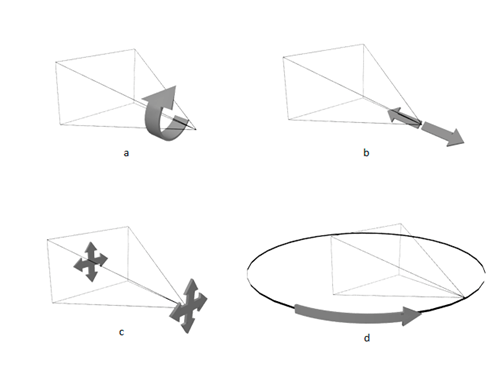
\includegraphics[width=0.5\textwidth]{./Cap5_vmt/vmtengine-cameramove.png}
  \caption{Movimientos de cámara. a) \emph{Roll} b) \emph{Dolly} c) \emph{Pan} d) \emph{Orbit}}%imagen nuestra no hay que referenciar%
  \label{fig:VMT-CameraMove}
\end{figure}

Aparte de estos parámetros de ubicación, también existe el parámetro \emph{Field Of View (FOV)} o campo de vista que es el ángulo de apertura de la cámara. Para el caso de cámaras que representan proyectores, este parámetro debe coincidir con el ángulo de apertura del proyector para ajustar correctamente las escenas con respecto a lo que muestra la cámara en pantalla.
Mediante estas operaciones es que las cámaras virtuales de \emph{VMT} ajustan sus parámetros para que la proyección de objetos tridimensionales coincida con las superficies proyectadas.
Hay que destacar que las cámaras proveen un punto de vista solo para los elementos tridimensionales. Los \emph{quads}, que como se mencionó son contrucciones bidimensionales, no dependen del punto de vista de la cámara y se representan en un sector de la pantalla relativo a esta. Es por esto que los \emph{quads} no alteran su posición en pantalla al ajustar los parámetros de la cámara.

Los \emph{quads} se pueden organizar en grupos, y estos pertenecen a una o más capas. A su vez cada capa pertenece a una única cámara de manera de representar las zonas a cubrir por un solo proyector. Es posible aplicar una transformación inicial a una capa, la que se aplicará a todos los \emph{quads} o grupos de \emph{quads} contenidos en ella. Esto es útil para ajustar la proyección de los \emph{quads} en caso de mover el proyector levemente y que esta proyección deje de coincidir con las superficies, y provee la funcionalidad básica y de bajo nivel para el mecanismo de calibración bidimensional que se detallará más adelante.

Las texturas se asocian a grupos de \emph{quads}. Los grupos también permiten variar de forma limitada como se mapean las texturas a los \emph{quads} que los componen. Pueden ser mapeadas por cara en donde a cada uno de los \emph{quads} se le mapeará toda la textura, o también de forma plana, esto es que la textura sea mapeada al conjunto entero de \emph{quads} como si estos fueran trozos de un \emph{quad} de mayor tamaño.

\begin{figure}[H]
  \centering
    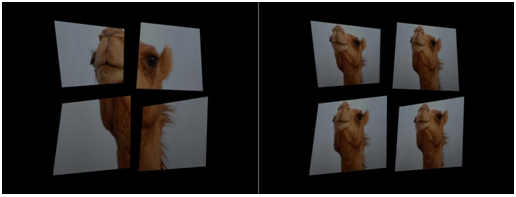
\includegraphics[width=0.7\textwidth]{./Cap5_vmt/vmtengine-maping.png}
  \caption{Izquierda: Proyección plana. Derecha: Proyección por cara.}%imagen nuestra no hay que referenciar%
  \label{fig:VMT-Projection}
\end{figure}

Con estas variantes de proyección se le dan más posibilidades a un artista para lograr los efectos utilizados normalmente en espectáculos de \emph{video mapping}.

La escena también contiene los efectos que se ejecutarán durante el espectáculo. Se aceptan como efectos la asignación de texturas en forma de imagen o video, ya sea a grupos de \emph{quads} u objetos tridimensionales, el \emph{fade} en un material desde un color inicial a otro final, y la animación de la posición de un objeto tridimensional de un origen a un destino en un lapso de tiempo dado.

El efecto de mapeo de texturas es el más básico pero también el más potente en cuanto a la gran cantidad de alternativas al momento de mapear texturas sobre superficies. La variedad y la complejidad de las texturas está en la creación de los recursos de imagen o video que se deseen mapear. Al permitirse mapear estas texturas sobre objetos tridimensionales no es necesario distorsionar la forma de los videos sino que será el motor quien los adaptará a la forma del objeto que está siendo mapeado. El efecto de \emph{fade} puede ser combinado en un objeto que ya disponga de una textura y así permitir por ejemplo su atenuación o resaltado. La duración del \emph{fade}, al igual que la de animación de posición, es configurable.

Cabe aclarar que el estado final de la escena y todos los objetos contenidos en ella será el que resulte luego de la finalización de los efectos. Por ejemplo, si un objeto es de color rojo, y tiene un efecto de \emph{fade} al azul aplicado, su color luego de la ejecución del efecto continuará siendo azul.

Como se mencionó anteriormente, una de las tareas principales es la representación en pantalla o la proyección de los elementos gráficos. La implementación del dibujado se realiza en un bucle principal de la aplicación encargado de actualizar todos los objetos de la escena de ser necesario, procesar los eventos pendientes y finalmente dibujar el resultado. Este es un proceso cíclico que se repite varias veces por segundo.
En cada uno de estos ciclos se generan los cuadros que son las imágenes que se muestran como resultado final.
Para dar la ilusión de continuidad, la frecuencia de estos ciclos debe ser alta. En el caso de \emph{VMT} ésta se predetermina en 60 ciclos por segundo aunque alcanzar esta frecuencia dependerá de varios factores como la cantidad de \emph{quads}, tamaño de texturas utilizadas, capacidad de procesamiento y memoria de los equipos.
Si esta frecuencia se encuentra muy por debajo de los 60 ciclos, la reproducción del espectáculo no será fluida y se podrán percibir saltos o pausas al reproducirlo.
Para que esta frecuencia efectivamente se logre es necesario que el procesamiento de cada uno de los ciclos del bucle principal sea eficiente en cuanto al costo de procesamiento en cada tarea u operación. A continuación se muestra un pseudo-código del bucle principal de dibujado y se analizan cada una de las acciones que se toman, su impacto en cuanto al rendimiento del programa y las medidas que se tomaron para su optimización:

\begin{algorithm}
    \caption{Pseudo-código bucle de dibujado.}
    \label{alg:mainLoop}
    \begin{algorithmic}
      \State $posicionarCamara();$
      \ForAll{objeto3d $obj$ en la escena}
        \ForAll{cara $c$ de $obj$}
             \State $mat = cargarMaterial(obj);$
             \State $c.dibujar(mat);$
         \EndFor
      \EndFor

      \State $resetCamara();$
      \ForAll {quad $q$ en la escena}
         \State $mat = q.cargarMaterial();$
         \State $q.dibujar(mat);$
      \EndFor
    \end{algorithmic}
\end{algorithm}


Un bucle de este estilo cuenta con varios cuellos de botella.
La carga de materiales implica copiar una textura a la zona de la memoria de video correspondiente para utilizarla. Esto podría ser un proceso lento si no se disponen las texturas precargadas en memoria. Es por esta razón que las texturas se cargan desde un comienzo en memoria y luego se utilizan referencias para identificarlas y asociarlas a una unidad de textura de \emph{OpenGL}\footnote{www.opengl.org/wiki/Texture} para que se encuentre disponible.
Otra optimización pasa por hacer uso de \emph{shaders} para el cálculo del resultado visual final.
La visualización fluida de un espectáculo de \emph{video mapping} es difícil de predecir ya que, como se puede ver en el pseudo-código, los tiempos de ejecución dependen de la cantidad de materiales, caras, objetos y \emph{quads} incluidos en la escena.
Si se utilizan videos en las texturas, la compresión y resolución de estos también afecta la fluidez del espectáculo. Preferentemente deberían estar descomprimidos o con una baja tasa de compresión. El mismo problema ocurre con formatos de imágenes comprimidas, pero teniendo un menor impacto en el rendimiento de la reproducción del espectáculo.
%Esto no es verdad ya que hay codecs que son ideales para real time%

\subsection{Multi proyector}

Uno de los puntos fuertes de \emph{VMT} es la posibilidad de editar y visualizar un espectáculo de \emph{video mapping} utilizando más de un proyector. El soporte de múltiples proyectores puede lograrse de diferentes formas de distribución.

La forma más sencilla de conectar varios proyectores es con más de una salida de video desde la mismo computadora. Esto es posible mediante una tarjeta de video con salida múltiple, conectando cada proyector a cada una de estas salidas. Luego, se configura el sistema operativo para que extienda la resolución en las múltiples salidas y de esta forma se dispondrá de un área de trabajo mayor. Los diferentes sectores del área de trabajo serán desplegados por los proyectores conectados.
\emph{VMT} permite, al inicio de un espectáculo, indicar la resolución y la posición en pantalla en donde se desplegará. Controlando estos parámetros se permiten distintas variaciones en la configuración de la aplicación y en la disposición de los proyectores.

Otra forma de lograr varias salidas es conectando un dispositivo como las tarjetas \emph{DualHead2Go} o \emph{TripleHead2Go}\footnote{www.matrox.com/graphics/en/products/gxm/} y de esta manera conectar dos o tres proyectores a partir de una única salida de la tarjeta de video. El resultado es similar al anterior, extendiendo el área de trabajo a la resolución duplicada o triplicada.

Estas variantes en la forma de conectar los proyectores son útiles cuando se desea proyectar sobre una superficie tan extensa que un solo proyector no pueda abarcarla completamente, ya que como se menciona, el área de trabajo o escritorio es extendido para abarcar la cantidad de proyectores conectados al computador único, con la restricción de que están todos organizados de forma contigua. En cambio, si queremos proyectar sobre zonas de la escena contiguas entre si, lo ideal es contar con proyectores conectados a nodos distribuidos e independientes tanto al momento de la producción del espectáculo como al de su ejecución.

\begin{figure}[H]
  \centering
    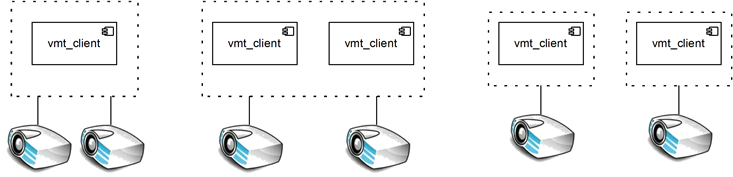
\includegraphics[width=0.8\textwidth]{./Cap5_vmt/vmt_multiProjector.png}
  \caption{Escenarios posibles de múltiples proyectores en VMT}%imagen nuestra no hay que referenciar%
  \label{fig:VMT-MultiProjector}
\end{figure}


En \emph{VMT}, el escenario descrito se implementa teniendo una instancia de \emph{VMT} maestro que orquestará toda la ejecución del espectáculo, y varias instancias de \emph{VMT} esclavo con uno o mas proyectores conectados. Para modelarlo en la herramienta se agregan los proyectores a la escena, asignando las propiedades para cada uno en particular, y luego se define la red de nodos de \emph{VMT} esclavo con la información de conectividad necesaria y su asociación al proyector que tiene conectado el nodo. La comunicación entre maestro y esclavos se realiza sobre \emph{OSC}, protocolo construido sobre \emph{UDP} para \emph{IP} vía \emph{Ethernet} o \emph{WiFi}. Por la naturaleza del protocolo \emph{UDP}, es preferible contar con conexiones cableadas en lugar de inalámbricas dada la alta tasa de pérdida de paquetes que existe en este tipo de redes, lo cual podría causar desincronización de algunos nodos esclavos. \emph{OSC} también permite a cualquier aplicación capaz de enviar mensajes \emph{OSC} y que conozca el formato de los mismos para \emph{VMT}, controlar los esclavos y por consiguiente lo que se proyecta en los correspondientes proyectores.

%%% VA ACÁ Esta información es necesaria para establecer el canal de comunicación con el proceso remoto y deducir que información se enviará al nodo en base a su cámara asociada. Recordar que las \emph{layers} están asociadas a una y solo una cámara, por lo cuál si un efecto está aplicado sobre un \emph{quad} o grupo de \emph{quads}, el mismo deberá ser propagado al nodo cuya cámara sea la que los contiene. Referente a los efectos aplicados sobre objetos tridimensionales, estos serán enviados a todos los nodos ya que todas las cámaras tienen visibilidad de la escena tridimensional, aunque esta sea desde perspectivas diferentes.

\subsection{Calibración}

\emph{VMT} ofrece la capacidad de calibrar las cámaras para que la proyección reflejada por los proyectores se corresponda y ajuste a la geometría de la escena.
Como se mencionó anteriormente, \emph{VMT} permite trabajar simultáneamente de forma bidimensional y tridimensional. Cada uno de estos modos de trabajo requiere distintos mecanismos de calibración.

La calibración bidimensional se basa en ajustar todos los \emph{quads} de una \emph{layer} de forma conjunta.
Inicialmente, al preparar el espectáculo, los \emph{quads} son posicionados en pantalla para cubrir las áreas de interés a proyectar. Luego de este posicionamiento inicial, cualquier movimiento de los proyectores causará que se desajuste simultáneamente la proyección de todos los \emph{quads}. Si ocurre un desajuste se hace necesario reposicionar los \emph{quads} para que vuelvan a cubrir las áreas a proyectar.
\emph{VMT} ofrece la posibilidad de ajustar todos los \emph{quads} pertenecientes a una misma \emph{layer} de forma simultánea aplicando una homografía. Esta transformación es la que ocurre naturalmente en la proyección al variar la posición u orientación del mismo por lo tanto es necesario aplicar la transformación inversa para que los \emph{quads} se ajusten nuevamente a las superficies.

Por otra parte, la calibración tridimensional se basa en hacer coincidir los parámetros de posición, orientación y proyección de las cámaras con los de los proyectores físicos. Este ajuste de parámetros se realiza manualmente por el usuario, utilizando los modos de movimientos de cámara antes mencionados. Esta calibración es necesario hacerla de forma independiente en cada una de las cámaras y proyectores.

Cabe acotar que en los escenarios de múltiples proyectores este modelo de calibración asume que existe un solo proyector conectado a cada nodo, si bien es posible conectar más de uno mediante placas especializadas como se vio anteriormente. Sólo se podrán modificar los parámetros a la única cámara asociada al nodo en el modelo \emph{VMT}, por lo cuál en caso de ser más de un proyector no será posible ajustar los parámetros de todos. Los planos de imagen tampoco podrían coincidir, si no están posicionados exactamente paralelos.


\section{Interfaz gráfica de usuario}

Para la estructura definida de escena o espectáculo, la interfaz gráfica cuenta con formularios sencillos de altas, bajas y modificaciones para todos los tipos de objetos existentes. Se diseñó en base a barras de herramientas flotantes de forma de poder tener visibilidad de la escena en todo momento y observar así como los cambios efectuados impactan sobre ella.

\begin{figure}[H]
  \centering
    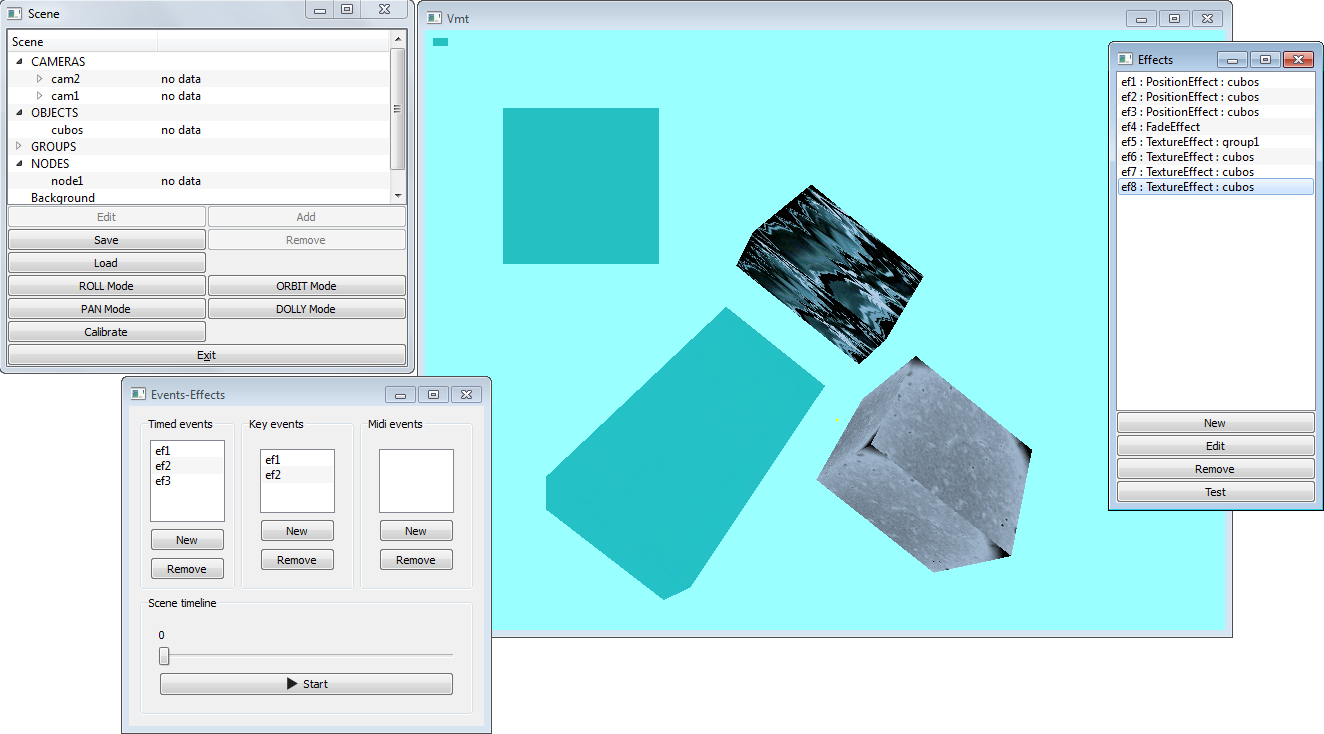
\includegraphics[width=0.8\textwidth]{./Cap5_vmt/vmt_todo.png}
  \caption{Vista general de la interfaz de usuario de \emph{VMT}}
  \label{fig:VMT-MainWindow}
\end{figure}

Al inicio se cuenta con una vista gráfica de la escena desde el punto de vista de la cámara activa, una vista de los objetos contenidos en la escena, la lista de definición de efectos y una línea de tiempo con las listas de efectos por tiempo, por evento de teclado y evento \emph{MIDI}.
En la ventana de escena se manejan los objetos bidimensionales y tridimensionales, cámaras, luces, capas y los nodos distribuidos del espectáculo. También es desde donde se ejecuta la calibración de las cámaras virtuales. En la visualización de la escena se ofrecen diferentes modos de cámara que permite girar u orbitar alrededor del centro, o moverse en cada uno de los ejes.

\begin{figure}[H]
  \centering
    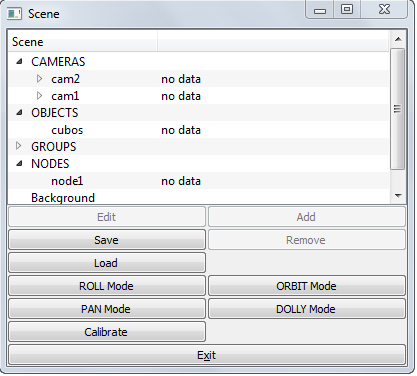
\includegraphics[width=0.5\textwidth]{./Cap5_vmt/vmt_scene.png}
  \caption{Ventana para manejar la escena}
  \label{fig:VMT-SceneWindow}
\end{figure}

\subsection{Cámaras, capas y \emph{quads}}
Las cámaras tienen todas las propiedades usuales que se pueden encontrar en paquetes de \emph{software} de animación tridimensional como ser posición, \emph{eye}, \emph{up}, \emph{FOV}, aspecto, \emph{near}\footnote{explicar near}, \emph{far}\footnote{explicar far}.

\begin{figure}[H]
  \centering
    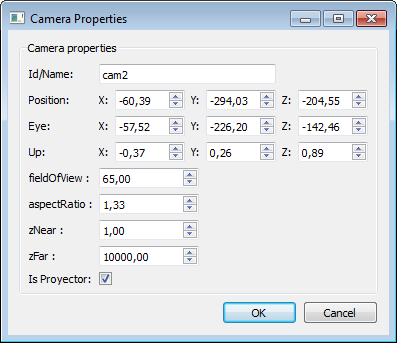
\includegraphics[width=0.5\textwidth]{./Cap5_vmt/vmt_cameraProperties.png}
  \caption{Diálogo de propiedades de cámara}
  \label{fig:VMT-CameraProperties}
\end{figure}

Las cámaras y proyectores son modeladas con el elemento cámara diferenciando mediante la propiedad \emph{isProjector}. De esta forma un elemento cámara se utiliza para simular la vista de un observador, mientras que un proyector será la vista de la proyección en perspectiva del espectáculo.
Los tipos de movimiento de la cámara activa son los descriptos anteriormente.

\begin{figure}[H]
  \centering
    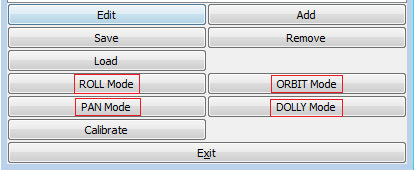
\includegraphics[width=0.5\textwidth]{./Cap5_vmt/vmt_SceneBotonera.png}
  \caption{Acciones para seleccionar modo de movimiento de la cámara activa}
  \label{fig:VMT-CameraActions}
\end{figure}

Una vez seleccionado el modo de la cámara, manteniendo presionado el botón izquierdo del ratón al moverlo se mueve la cámara acorde al modo seleccionado.
Cada cámara es a su vez un contenedor de \emph{layers}. Su propósito es manejar todo lo relacionado al mapeo sobre estructuras bidimensionales, y por ello son los contendores de \emph{quads} bidimensionales sobre los cuales se pueden realizar todas las operaciones y efectos disponibles.

\begin{figure}
	\begin{center}
		\begin{tabular}[c]{cc}
			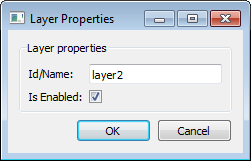
\includegraphics[width=0.3\textwidth]{./Cap5_vmt/vmt_layerProperties.png}
				&        
			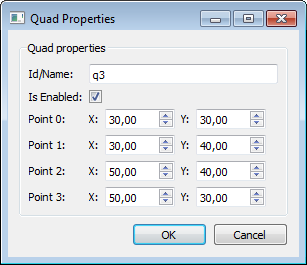
\includegraphics[width=0.3\textwidth]{./Cap5_vmt/vmt_quadProperties.png}
		\end{tabular}
	\end{center}
	\caption{Propiedades de los objetos \emph{Layer} y \emph{Quad}}
	\label{fig:VMT-LayerQuadProperties}
\end{figure}

Tanto el \emph{quad} como la \emph{layer} tienen propiedades editables en tiempo de edición o durante el espectáculo para mostrarse u ocultarse completamente. Si se oculta una \emph{layer}, todos los \emph{quads} contenidos en ella también serán ocultados. En caso de mostrarla, todos los \emph{quads} visibles volverán a desplegarse.

\subsection{Objetos tridimensionales}

Se permite agregar a la escena objetos tridimensionales con formato de malla triangular del tipo \emph{3DS}.

\begin{figure}[H]
  \centering
    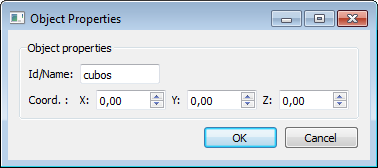
\includegraphics[width=0.5\textwidth]{./Cap5_vmt/vmt_objectProperties.png}
  \caption{Diálogo de propiedades de objeto tridimensional}
  \label{fig:VMT-ObjectProperties}
\end{figure}

\subsection{Efectos}

Se proveen ventanas flotantes tanto para la definición de efectos como para la asociación con sus disparadores como ser un instante específico, un evento de teclado o un evento \emph{MIDI}.

Si un efecto es definido para ser desplegado en un instante dado este se podrá visualizar cuando la línea de tiempo pase por ese instante. En caso de ser definido por evento este será visualizado cada vez que el evento asociado suceda, sea un evento de teclado o \emph{MIDI}.
Los efectos de posición son aplicables únicamente a objetos tridimensionales y permiten animar el objeto trasladándolo de una posición inicial a una final.

\begin{figure}[H]
  \centering
    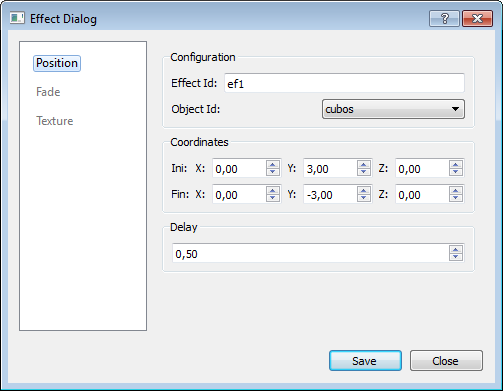
\includegraphics[width=0.5\textwidth]{./Cap5_vmt/vmt_EfectDialog1.png}
  \caption{Diálogo de definición de efecto de tipo posición}
  \label{fig:VMT-EffectPossition}
\end{figure}

Los efectos de \emph{fade} sólo son aplicables a grupos de \emph{quads} y lo que permiten es pintar todos los \emph{quads} del grupo de un color inicial e ir pasando por toda la gama de colores intermedios hasta llegar al color final. Para la selección de colores se utiliza un diálogo específico para ese propósito. También es posible definir la duración del efecto.

\begin{figure}[H]
  \centering
    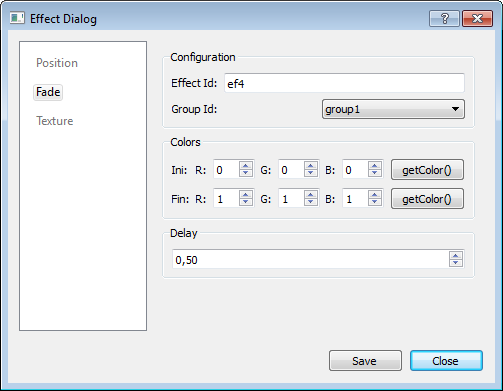
\includegraphics[width=0.5\textwidth]{./Cap5_vmt/vmt_EfectDialog2.png}
  \caption{Diálogo de definición de efecto de tipo \emph{fade}}
  \label{fig:VMT-EffectFade}
\end{figure}

Los efectos de tipo textura son aplicables tanto a grupos de quads como a objetos tridimensionales. Se pueden definir texturas de tipo Imagen o Video. En ambos casos es necesario proporcionar el camino al archivo multimedia correspondiente. Para el caso especifico de un efecto de textura asociado a un objeto tridimensional, es necesario proporcionar además la cara o conjunto de caras sobre los cuales se va a mapear el efecto de tipo textura definido.

\begin{figure}[H]
  \centering
    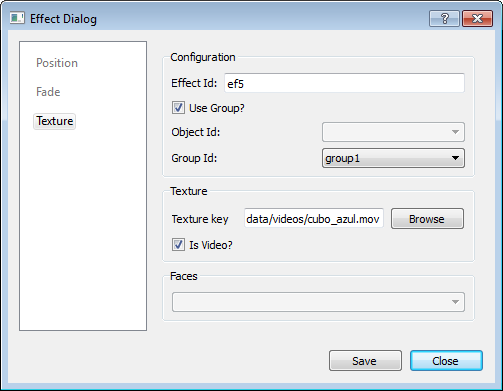
\includegraphics[width=0.5\textwidth]{./Cap5_vmt/vmt_EfectDialog3.png}
  \caption{Diálogo de definición de efecto de tipo textura aplicada a un grupo.}
  \label{fig:VMT-EffectTexture}
\end{figure}

\begin{figure}[H]
  \centering
    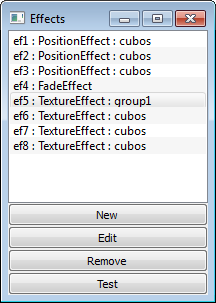
\includegraphics[width=0.2\textwidth]{./Cap5_vmt/vmt_Efects.png}
  \caption{Lista de efectos definidos en la escena}
  \label{fig:VMT-EffectList}
\end{figure}

Es posible visualizar el efecto que se está creando presionando el botón \emph{Test} de la lista de efectos. Esto disparará la ejecución por una única vez del efecto seleccionado en la lista.

\subsection{Calibración}

El proceso de calibración en \emph{VMT} se basa en posicionar cuatro puntos de la superficie donde se proyecta y cuatro puntos de la capa contenedora de \emph{quads} para de esta forma calcular la matriz de transformación de la homografía que los hace corresponder.

\begin{figure}[H]
  \centering
    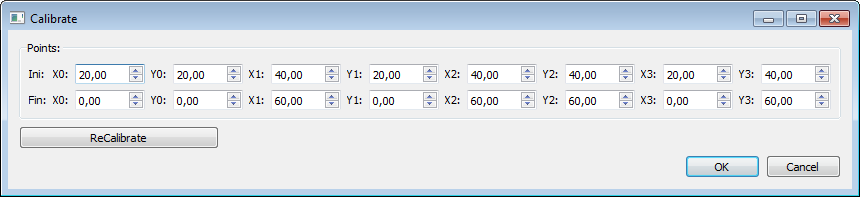
\includegraphics[width=0.6\textwidth]{./Cap5_vmt/vmt_Calibrate.png}
  \caption{Diálogo para configurar y ejecutar la calibración}
  \label{fig:VMT-Calib}
\end{figure}

Al ingresar en el modo calibración se muestra en la pantalla de edición cuatro puntos azules de destino y cuatro puntos rojos de origen junto con el diálogo de configuración de la calibración.
El diálogo posee controles para posicionar cada uno de los ocho puntos mostrados en pantalla. Se deberán posicionar los cuatro puntos de origen en regiones significativas de la capa donde hayan vértices de \emph{quads} preferiblemente alejados entre si. De esta forma se minimiza el error obtenido al calcular la matriz.
Los cuatro puntos de destino se deberán posicionar observando la proyección de estos sobre la superficie. Una vez los ocho puntos estén posicionados se podrá calcular y aplicar la nueva matriz de calibración presionando el botón \emph{OK}.
Mediante el botón \emph{ReCalibrate} se reestablece la calibración original, descartando los cambios realizados.

\subsection{Línea de tiempo}

Tanto para la fases de producción y previsualización del evento como para la ejecución o reproducción del espectáculo en vivo, es necesario contar con controles para el manejo de la línea de tiempo.

\begin{figure}[H]
  \centering
    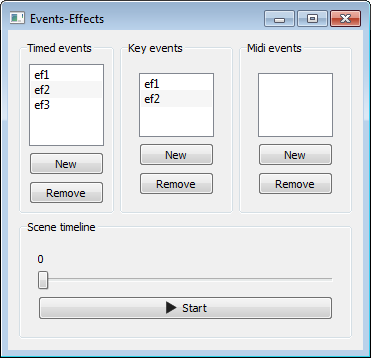
\includegraphics[width=0.5\textwidth]{./Cap5_vmt/vmt_events_effects.png}
  \caption{Diálogo con línea de tiempo y lista de efectos asociados a tiempo y eventos}
  \label{fig:VMT-Timeline}
\end{figure}

La aplicación provee una forma de iniciar el evento mediante la acción de \emph{Start}. Se provee una vista gráfica representada con una barra deslizante y una vista numérica para reflejar el avance en el tiempo en relación a la duración total del evento. Utilizando la barra deslizante es posible navegar por la línea de tiempo e iniciarla visualización del evento desde un instante cualquiera. Esto último es muy útil para la fase de pre-producción del espectáculo en la cual es muy común que el usuario se quiera concentrar en un lapso específico en el que se está trabajando.

Sobre la línea de tiempo se pueden observar las listas de eventos agrupados por tipo, pudiéndose asociar cualquiera de los eventos previamente definidos a un instante dado o a un código de evento a ser utilizado durante el espectáculo, ya sea de teclado o proveniente de dispositivos de entrada \emph{MIDI}.

\subsection{Nodos remotos}

Para modelar la red de nodos esclavos de \emph{VMT} en los cuales se conectarán proyectores remotos es preciso definir, para cada nodo, su dirección \emph{IP} y número de puerto en donde estarán configurados así como también la cámara definida en la escena que representará al proyector asociado.

\begin{figure}
	\begin{center}
		\begin{tabular}[c]{cc}
			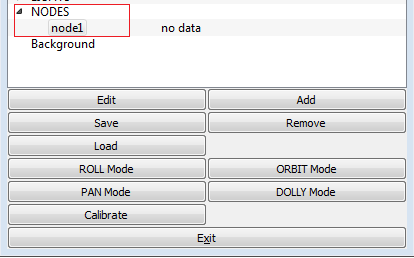
\includegraphics[width=0.3\textwidth]{./Cap5_vmt/vmt_nodeProperties_1.png}
				&        
			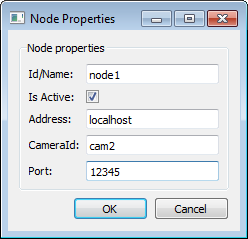
\includegraphics[width=0.3\textwidth]{./Cap5_vmt/vmt_nodeProperties_2.png}
		\end{tabular}
	\end{center}
	\caption{Lista de nodos y diálogo de propiedades de nodos}
	\label{fig:VMT-Nodes}
\end{figure}

\subsection{Escena en XML}
Se permite almacenar en archivos \emph{XML} estándar una representación de lo que se ha definido en la escena. Para la búsqueda de los archivos \emph{XML} se utilizan diálogos nativos para este propósito.

\begin{figure}[H]
  \centering
    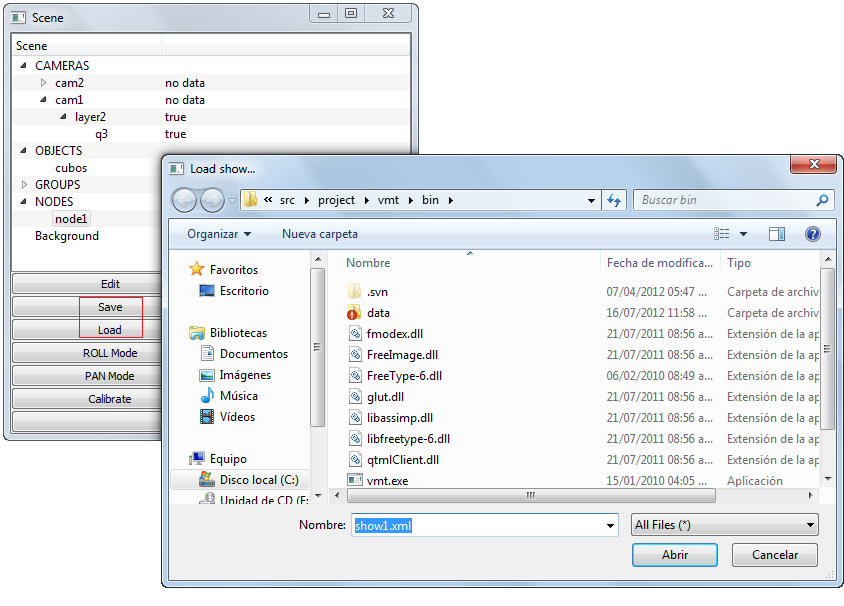
\includegraphics[width=0.5\textwidth]{./Cap5_vmt/vmt_loadShow.png}
  \caption{Diálogo para cargar y guardar archivos \emph{XML}.}
  \label{fig:VMT-XML}
\end{figure}

\section{Decisiones de implementación}
Para la implementación del módulo de interfaz gráfica se siguió el patrón \emph{Model-View-Controller (MVC)}\footnote{Explicar MVC}. Para cada ventana se generaron modelos que manejan los datos relevantes a cada una, impactando en el modelo general de la aplicación en caso de ser necesario.
Se utilizó \emph{Qt Framework} \cite{Qt-framework} como biblioteca de base para la creación de las ventanas, sus controles gráficos y manejo de la comunicación que ocurre entre ventanas y con los modelos de \emph{VMT}. También se hizo uso de la funcionalidad para internacionalización de las interfaces gráficas, las que por el momento están tomando valores por defecto en idioma inglés. \emph{Qt Framework} es multiplataforma por lo que puede ser utilizado en varios de los sistemas operativos más populares como \emph{Linux}, \emph{Mac OS X} y \emph{Windows}.

\section{Calibración NO VMT}
En este proyecto se desarrolla un método de calibración cuyo objetivo es obtener la posición del proyector con respecto a un sistema de coordenadas ubicado en un punto elegido relativo a la escena. Para ello se utiliza una superficie de calibración que puede existir ya en la escena o puede ser ubicada sobre ésta de forma temporal. Esta superficie de calibración deberá ser un plano rectangular en donde uno de los vértices será el centro de coordenadas que se desea determinar. La orientación del plano determinará la alineación del centro de coordenadas con sus ejes $X$ e $Y$ alineados con dos de los bordes del plano y el eje $Z$ perpendicular a éste. Se utiliza además un proyector asumiendo el modelo \emph{pinhole}\footnote{Ver sección con modelo \emph{pinhole}}.

Para encontrar el sistema de coordenadas buscado, se resuelve el problema opuesto que es encontrar la posición del punto que será origen del nuevo centro de coordenadas con respecto al centro de proyección ubicado dentro del proyector. Este método utiliza tres de los vértices de la superficie de calibración que formarán una base del nuevo sistema de coordenadas. Las medidas de la superficie de calibración son conocidas por lo que la distancia entre sus vértices también lo son. Desde el centro del proyector se proyectan rayos de luz, tres de los cuales pasan por los vértices de la superficie de calibración y también por el centro de proyección con coordenadas $(0, 0, 0)$. Para obtener la ecuación de estos rayos solo se precisa un punto distinto al origen. La ecuación de este punto puede ser obtenida utilizando las coordenadas en pantalla del píxel que se proyecta en cada vértice de la superficie de calibración.
%Traducir la imagen%
\begin{figure}[H]
  \centering
    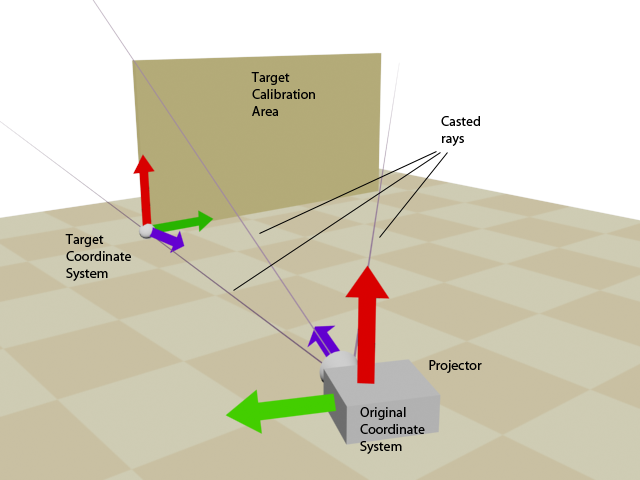
\includegraphics[width=0.7\textwidth]{./Cap2_videomapping/CalibrationSketch}
  \caption{Esquema de calibración.}
  \label{fig:CalibrationSketch}
\end{figure}
Usando las coordenadas en la pantalla de estos puntos y otros parámetros intrínsecos del proyector que son su resolución y el ángulo de proyección, es posible encontrar las coordenadas del punto con respecto al centro de proyección y por tanto la ecuación del rayo.
\[
a(t) = \vec{P} . t,	\mbox{ ecuación del rayo en dónde } \vec{P} \mbox{ es cualquier punto del rayo.}
\]
\[
\begin{cases}
P(X) = \frac{res_x}{2} - s_x \\
P(Y) = \frac{res_y}{2} - s_y \\
P(Z) = \frac{res_y}{2 \cdot \tan \frac{fov_y}{2}}
\end{cases}
\]
en donde $s_x$ y $s_y$ son las coordenadas del \emph{pixel}, $res_x$ y $res_y$ son la resolución horizontal y vertical del proyector y $fov_y$ es el ángulo de proyección vertical del proyector.

Aplicando esta ecuación a cada uno de los puntos a determinar se obtienen las ecuaciones paramétricas de los tres rayos. Vale aclarar que estos puntos $P$ son puntos de los rayos pero no necesariamente coinciden con los vértices de la superficie de calibración. Queda hallar las coordenadas de los vértices determinando el parámetro $t$ para cada ecuación. Para hallar este parámetro se resuelve un sistema de ecuaciones utilizando las tres ecuaciones de los rayos y las distancias conocidas entre estos puntos.
% Sistema de ecuaciones %
\[
\begin{cases}
\lVert{a(t_0) - b(t_1)} = j\rVert \\
\lVert{b(t_1) - c(t_2)} = k\rVert \\
\lVert{c(t_2) - a(t_0)} = l\rVert
\end{cases}
\]
siendo $a$, $b$ y $c$ los rayos y $j$, $k$ y $l$ las distancias entre las parejas de puntos.
La solución será entonces los parámetros $t_0$, $t_1$ y $t_2$ que satisfacen el sistema de ecuaciones no lineal.
Una aproximación a esta solución se puede obtener utilizando métodos numéricos, por ejemplo, el método \emph{trust-region-dogleg}\cite{TrustRegionDogleg}.
Una vez hallados los valores para $t_0$, $t_1$ y $t_2$, las coordenadas de los vértices de la superficie de calibración son $a(t_0)$, $b(t_1)$ y $c(t_2)$.
La base para el sistema de coordenadas con origen en el punto $P$ es:
\[
x' = \frac{b(t_1) - a(t_0)}{\lVert b(t_1) - a(t_0) \rVert},\quad y' = \frac{c(t_2) - a(t_0)}{\lVert c(t_2) - a(t_0)\rVert},\quad z' = -x' \times y'
\]
La ubicación del proyector en este nuevo sistema se obtiene proyectando cualquiera de los rayos en la nueva base de coordenadas.

\section{Tratamiento de malla}

Para la generacion mallas manejables por nuestra herramienta VMT se desarrollo un componente que se ejecuta separadamente y que recibe como entrada la nube de puntos a procesar. Como salida se generan mallas triangulares en el formato estandard OBJ.

%Rearmar la prosa de este primer párrafo%
Para la implementación de este módulo se utilizan los algoritmos descriptos en el estado del arte que incluye \emph{VcgLib} y que forman parte del procesamiento de malla propuesto. Para visualizar y evaluar los resultados esperados fue utilizada la aplicación de código abierto para la manipulación de mallas tridimensionales en diferentes formatos \emph{MeshLab} \cite{MeshLab}. Particularmente se utilizan los algoritmos de muestreo \emph{Poisson-disk} para reducir y normalizar los puntos de la malla inicial, \emph{normal extrapolation} para el cálculo de normales y reconstrucción de superficies de Poisson para la reconstrucción de la malla final.

Esta aplicación cuenta con una sencilla y única ventana que recibe los parametros para la configuración de los algoritmos que se ejecutan en cada uno de los pasos del procesamiento.

\begin{figure}[H]
  \centering
    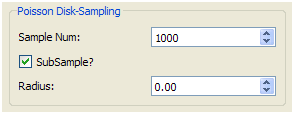
\includegraphics[width=0.5\textwidth]{./Cap2_videomapping/malla-poissongui.png}
  \caption{Configuración de parámetros del algoritmo \emph{Poisson-disk}}
  \label{fig:Mesh-PoissonGui}
\end{figure}

\begin{figure}[H]
  \centering
    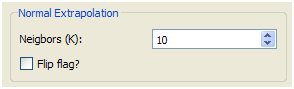
\includegraphics[width=0.5\textwidth]{./Cap2_videomapping/malla-normalextrapolation.png}
  \caption{Configuración de parámetros para reconstrucción de normales}
  \label{fig:Mesh-Extrapolation}
\end{figure}

\begin{figure}[H]
  \centering
    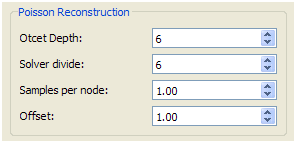
\includegraphics[width=0.5\textwidth]{./Cap2_videomapping/malla-poissonreconstruction.png}
  \caption{Configuración de parámetros para reconstruccion de malla de Poisson}
  \label{fig:Mesh-Normals}
\end{figure}


\subsection{Pruebas y resultados}

%Esta sección va dentro de lo que implementamos, recien aca salta que lo hicimos nosotros%

Para validar el correcto funcionamiento de esta técnica mediante los tres algoritmos descritos, fue utilizada una malla inicial de 5021 vértices y 9608 caras triangulares. Cabe destacar que si bien se ha mencionado que la malla de entrada debe ser simplemente una nube de puntos, se pueden utilizar mallas con caras, solo que estas serán ignoradas e incluso eliminadas de la malla de salida del primer paso del procesamiento (muestreo de \emph{Poisson-disk}).
Luego de experimentar con varios juegos de datos iniciales durante varias ejecuciones del procesamiento, se fijaron de manera personalizada para la malla de entrada algunos parámetros clave. Dado que la muestra inicial tiene alrededor de cinco mil puntos, fueron elegidas cinco mil muestras para el algoritmo de \emph{Poisson-disk}. Luego, para la extrapolación de normales se utilizan $K=15$ vecinos para la toma de decisiones locales de aproximación.
La aplicación de estos algoritmos resultó ser lo esperado en términos estructurales de cada malla procesada en cada uno de los pasos.
%Puede ir a trabajo futuro: No se llegó a procesar mallas de ambientes tridimensionales escaneados para luego ser mapeados con la herramienta.%

\begin{table}
\begin{center}
\begin{tabular}{|l||cc|} \hline
  Fase & Vértices & Caras \\
  Nube inicial & 5021 & 9608 \\
  Poisson-disk & 1776 & 0 \\
  Extrapolación Normales & 1776 & 0 \\
  Reconstrucción de Poisson & 1959 & 3910 \\ \hline %hay 1959 puntos en lugar de 1776, por que?%
\end{tabular}
\caption{Comparación de estructura de mallas de entrada y salida en cada fase}
\end{center}
\end{table}

\begin{figure}[H]
  \centering
    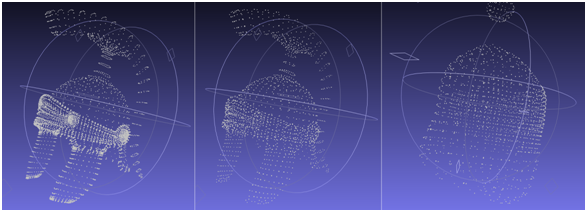
\includegraphics[width=0.8\textwidth]{./Cap2_videomapping/malla-nubepuntos.png}
  \caption{1) Nube de puntos inicial con 5021 vértices. 2) Resultado de muestreo \emph{Poisson-disk} con 1776 vértices. 3) Luego de extrapolar normales y reconstruir la malla con 1959 vértices y 3910 caras.}
  \label{fig:Mesh-Results}
\end{figure}
 
%Se observaron buenos tiempos computacionales de respuesta. Si bien la malla utilizada no es de un tamaño considerable, estamos hablando de algoritmos de orden relativamente alto.%
